\documentclass{beamer}
\usepackage{beamerthemesplit}
\usepackage{wrapfig}
\usetheme{SPbGU}
\usepackage{pdfpages}
\usepackage{amsmath}
\usepackage{cmap} 
\usepackage[T2A]{fontenc} 
\usepackage[utf8]{inputenc}
\usepackage[english,russian]{babel}
\usepackage{indentfirst}
\usepackage{amsmath}
\usepackage{tikz}
\usepackage{multirow}
\usepackage[noend]{algpseudocode}
\usepackage{algorithm}
\usepackage{algorithmicx}
\usetikzlibrary{shapes,arrows}
\usepackage{fancyvrb}
\usepackage{appendixnumberbeamer}
\usepackage[font={scriptsize,it}]{caption}
\usepackage[table]{xcolor}

\usepackage{tikz}
\usetikzlibrary{arrows,automata}
\usepackage[latin1]{inputenc}
\usepackage{changepage}
\usepackage{nicematrix}

\newtheorem{rutheorem}{Теорема}
\newtheorem{ruproof}{Доказательство}
\newtheorem{rudefinition}{Определение}
\newtheorem{rulemma}{Лемма}

\beamertemplatenavigationsymbolsempty

% То, что в квадратных скобках, отображается внизу по центру каждого слайда. 
\title[Разработка алгоритма RPQ]{Разработка алгоритма для задачи достижимости с регулярными ограничениями}

% То, что в квадратных скобках, отображается в левом нижнем углу. 
\institute[СПбГУ]{}

% То, что в квадратных скобках, отображается в левом нижнем углу.
\author[Денис Порсев]{Порсев Денис Витальевич, 19.Б10-мм}
 
\begin{document}
{
\setbeamertemplate{footline}{}
% Лого университета или организации, отображается в шапке титульного листа
\begin{frame}
  
\includegraphics[width=1.4cm]{pictures/SPbGU_Logo.png}
\vspace{-35pt}
\hspace{-10pt}
\begin{center}
   \begin{tabular}{c}
        \scriptsize{Санкт-Петербургский государственный университет} \\
        \scriptsize{Кафедра системного программирования}
    \end{tabular}
\titlepage
\end{center}

\btVFill

{\scriptsize
  % У научного руководителя должна быть указана научная степень
   {\bfseries Научный руководитель:} к.ф.-м.н., Григорьев С.В., доцент кафедры информатики \\
 }
\begin{center}
  \vspace{5pt}
  \scriptsize{Санкт-Петербург\\
                 2022}
  \end{center}

\end{frame}
}

\begin{frame}[fragile]  
  \frametitle{Графовые запросы}
  \noindent\begin{minipage}{0.59\textwidth}
  \begin{itemize}
    \item Графовое представление данных
    \begin{itemize}
        \item Метки на ребрах
        \item Формальные ограничения
    \end{itemize}
    \item Регулярные запросы к графовым БД
    \begin{itemize}
        \item Достижимость и обход графа
        \item Поиск путей в графе
        \item Путь ограничен регулярной грамматикой
    \end{itemize}
  \end{itemize}
  \end{minipage}
  \noindent\begin{minipage}{0.4\textwidth}
  \begin{figure}[h!]
      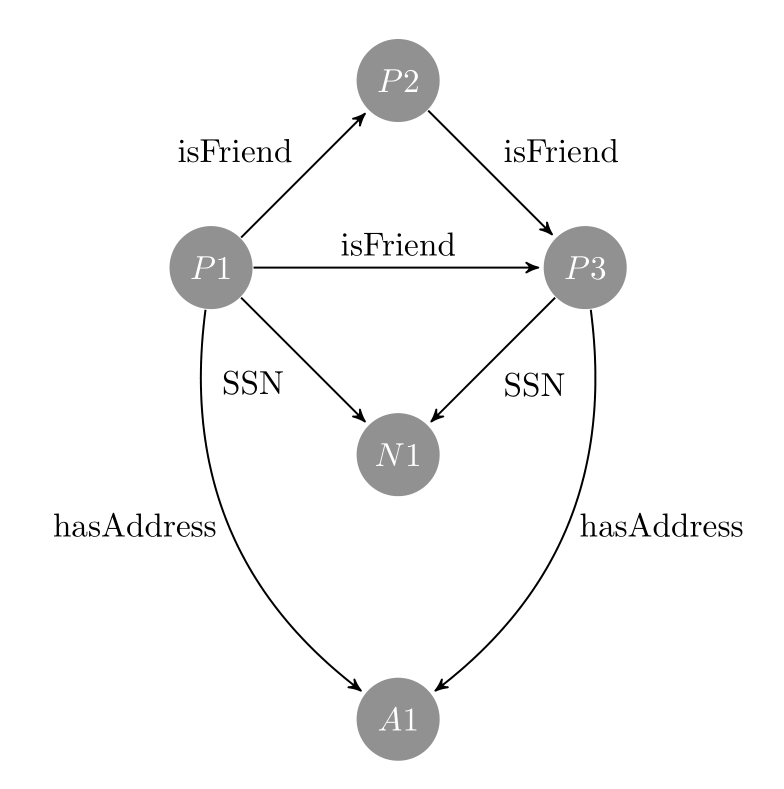
\includegraphics[width=1\linewidth]{pictures/intro_graph.PNG}
      \caption{Представление в виде графа}
  \end{figure}
\end{minipage}
\end{frame}

\begin{frame}[fragile]  
  \frametitle{Мотивация создания алгоритма}
  \noindent\begin{minipage}{1\textwidth}
  \begin{itemize}
    \item Регулярные запросы активно используются на практике
    \begin{itemize}
        \item В языках запросов: SPARQL v1.1, Cypher и др. 
        \item Существующие подходы неэффективны на различных графах
    \end{itemize}
    \item Новый подход: линейная алгебра
    \begin{itemize}
        \item Использование разреженной матрицы смежности
        \item Основные подходы к регулярным запросам используют BFS
        \item BFS выражен в терминах линейной алгебры
        \item SuiteSparse:GraphBLAS --- реализация примитивов линейной алгебры
    \end{itemize}
    
    \item Подготовка к запросам с контекстно-свободными ограничениями

  \end{itemize}
  \end{minipage}
  \noindent\begin{minipage}{0.4\textwidth}
  
\end{minipage}
\end{frame}



% Обязательный слайд: четкая формулировка цели данной работы и постановка задачи
% Описание выносимых на защиту результатов, процесса или особенностей их достижения и т.д.
\begin{frame}
  \frametitle{Постановка задачи}
  \textbf{Цель:} разработать алгоритм для задачи достижимости с регулярными ограничениями (RPQ) для нескольких стартовых вершин

  \textbf{Задачи:}
  \begin{itemize}
    \item Провести обзор алгоритмов RPQ и методов решения задачи
    \item Разработать матричный алгоритм, решающий задачу регулярной достижимости
    \item Реализовать разработанный алгоритм
    \item Провести экспериментальное исследование алгоритма
  \end{itemize}
\end{frame}
            
%Идеально, если есть по одному слайду на каждую поставленую задачу

\begin{frame}
  \frametitle{Задача достижимости с регулярными ограничениями}
  \begin{rudefinition}[Задача регулярной достижимости в графе для нескольких стартовых вершин]
    Имеется:
    \begin{itemize}
        \item Регулярный язык $\mathcal{R}=\langle Q, \Sigma, P, F, Q_{src} \rangle$
        \item Направленный помеченный граф $\mathcal{G}=\langle V, E, L \rangle$
        \item Множество начальных вершин $V_{src}\subset V$
    \end{itemize}
    Постановка задачи 1:
    \begin{itemize}
        \item Найти множество $\{w~|~\exists$ путь $\pi = (e_1, \dots, e_n), e_k = (v_k, l_k, v_{k+1})$, т.ч. $ L(\pi)=(l_1l_2 \dots l_n) \in L(\mathcal{R})$, $v_1 \in V_{src}, w \in V\}$
    \end{itemize}
    Постановка задачи 2:
    \begin{itemize}
        \item Найти множество пар $\{(v, w)~|~\exists$ путь $\pi$, т.ч. $ L(\pi)=(l_1l_2 \dots l_n) \in L(\mathcal{R})$, $v_1 \in V_{src}, w \in V\}$
    \end{itemize}
  \end{rudefinition}
\end{frame}


\begin{frame}[fragile]
  \frametitle{Основные алгоритмы RPQ}
  Два основных подхода:
  \begin{itemize}
    \item Алгоритм $\alpha{\text -}RA$, реляционная алгебра
    \item Использование FA, конечные автоматы
  \end{itemize}
\end{frame}

\begin{frame}[fragile]
  \frametitle{Основные алгоритмы RPQ: Использование $FA$}
  Идея:
  \begin{itemize}
    \item Регулярный запрос представляется в виде автомата $\mathcal{R}$
    \item Граф представляется в виде автомата $\mathcal{G}$
    \item Пересечение $\mathcal{R}$ и $\mathcal{G}$ содержит информацию о достижимых вершинах
  \end{itemize}
  Оптимизация:
  \begin{itemize}
    \item Матричный BFS синхронно по $\mathcal{R}$ и $\mathcal{G}$
  \end{itemize}
  \vspace{2em}
  \begin{center}
      $Q_1 = (sameAs \cdot isLocated)^+$
  \end{center}
  \noindent\begin{minipage}{1\textwidth}
  \begin{figure}
  \vspace{1em}
    \begin{tikzpicture}[->,>=stealth',shorten >=1pt,auto,node distance=2.8cm,semithick]
    \node[state, initial] (q1) {$q_1$};
    \node[state,  right of=q1] (q2) {$q_2$};
    \node[state, accepting, right of=q2] (q3) {$q_3$};
    \draw (q1) edge[below] node{sameAs} (q2)
    (q2) edge[below] node{isLocated} (q3)
    (q3) edge[bend right, above] node{sameAs} (q2);
    \end{tikzpicture}
  \vspace{1em}
  \caption{Представление регулярного запроса в виде автомата}
  \end{figure}
  \end{minipage}
\end{frame}

\begin{frame}[fragile]
  \frametitle{Разработанный алгоритм}
Входные данные: $\mathcal{R}, \mathcal{G}, V_{src}$

Выходные данные: $\mathcal{P}$ - матрица достижимых пар вершин
  \begin{itemize}
      
      \item Посимвольно декомпозируем в булевые матрицы $Bool_{\mathcal{R}_a}$ и $Bool_{\mathcal{G}_a}$
      
      \item Cинхронизируем обход с помощью следующей матрицы
      \begin{equation}
\mathfrak{D} = 
  \left[
    \begin{matrix}
        Bool_{\mathcal{R}_a} & 0\\
        0 & Bool_{\mathcal{G}_a}
    \end{matrix}
  \right]
\end{equation}
    \item Строим матрицу с начальными вершинами, которая будет хранить найденные во время обхода вершины
    \begin{equation}
M^{k \times (k + n)} =
  \left[
    \begin{matrix}
        Id_k & Matrix_{k \times n }
    \end{matrix}
  \right]
\end{equation}
    
    \item Пока $M$ меняется:
\begin{itemize}
    \item Перемножаем $M \times \mathfrak{D}$ для получения новых вершин
    \item Переставляем строчки в $M$ для преобразования к начальному виду
    \item Записываем найденные вершины в $\mathcal{P}$
\end{itemize}
  \end{itemize}
\end{frame}

\begin{frame}[fragile]
  \frametitle{Условия эксперимента}
  Оборудование:
  \begin{itemize}
      \item Intel Core i7-10750H $6\times2.60$ GHz
      \item 16 Gb DDR4 RAM
  \end{itemize}
  
  \noindent\begin{minipage}{0.5\textwidth}
  \begin{table}[!ht]
    \centering
    \begin{tabular}{|l|l|l|}
    \hline
    Graph & \# Vertices & \# Edges \\ \hline
        core & 1 323 & 2 752 \\ \hline
        enzyme & 48 815 & 86 543 \\ \hline
        eclass & 239 111 & 360 248 \\ \hline
        go & 582 929 & 1 437 437 \\ \hline
    \end{tabular}
    \caption{Графы}\label{table1a}
\end{table}
  \end{minipage}
  \noindent\begin{minipage}{0.45\textwidth}
  \begin{table}[!ht]
    \centering
    \begin{tabular}{|l|l|l|}
    \hline
    Name & Query \\ \hline
        Q_1 & a^*\\ \hline
        Q_2 & a$\cdot$b^*\\ \hline
        Q_3 & a$\cdot$b^*$\cdot$c^*\\ \hline
        Q_4 & (a|b)^*\\ \hline
        Q_5 & a$\cdot$b^*$\cdot$c\\ \hline
        Q_6 & a^*$\cdot$b^*$\cdot$c\\ \hline
        Q_7 & a$\cdot$b$\cdot$c^*\\ \hline
        Q_8 & a?$\cdot$b^*\\ \hline
        Q_9 & (a|b)^+\\ \hline
        Q_{10} & (a|b)^+$\cdot$c^*\\ \hline
        Q_{11} & a$\cdot$b\\ \hline
    \end{tabular}
    \caption{Шаблоны запросов}\label{table1a}
\end{table}
\end{minipage}

\end{frame}

\begin{frame}[fragile]
  \frametitle{Экспериментальное исследование (SS)}
  \noindent\begin{minipage}{0.95\textwidth}
  \begin{figure}[h!]
      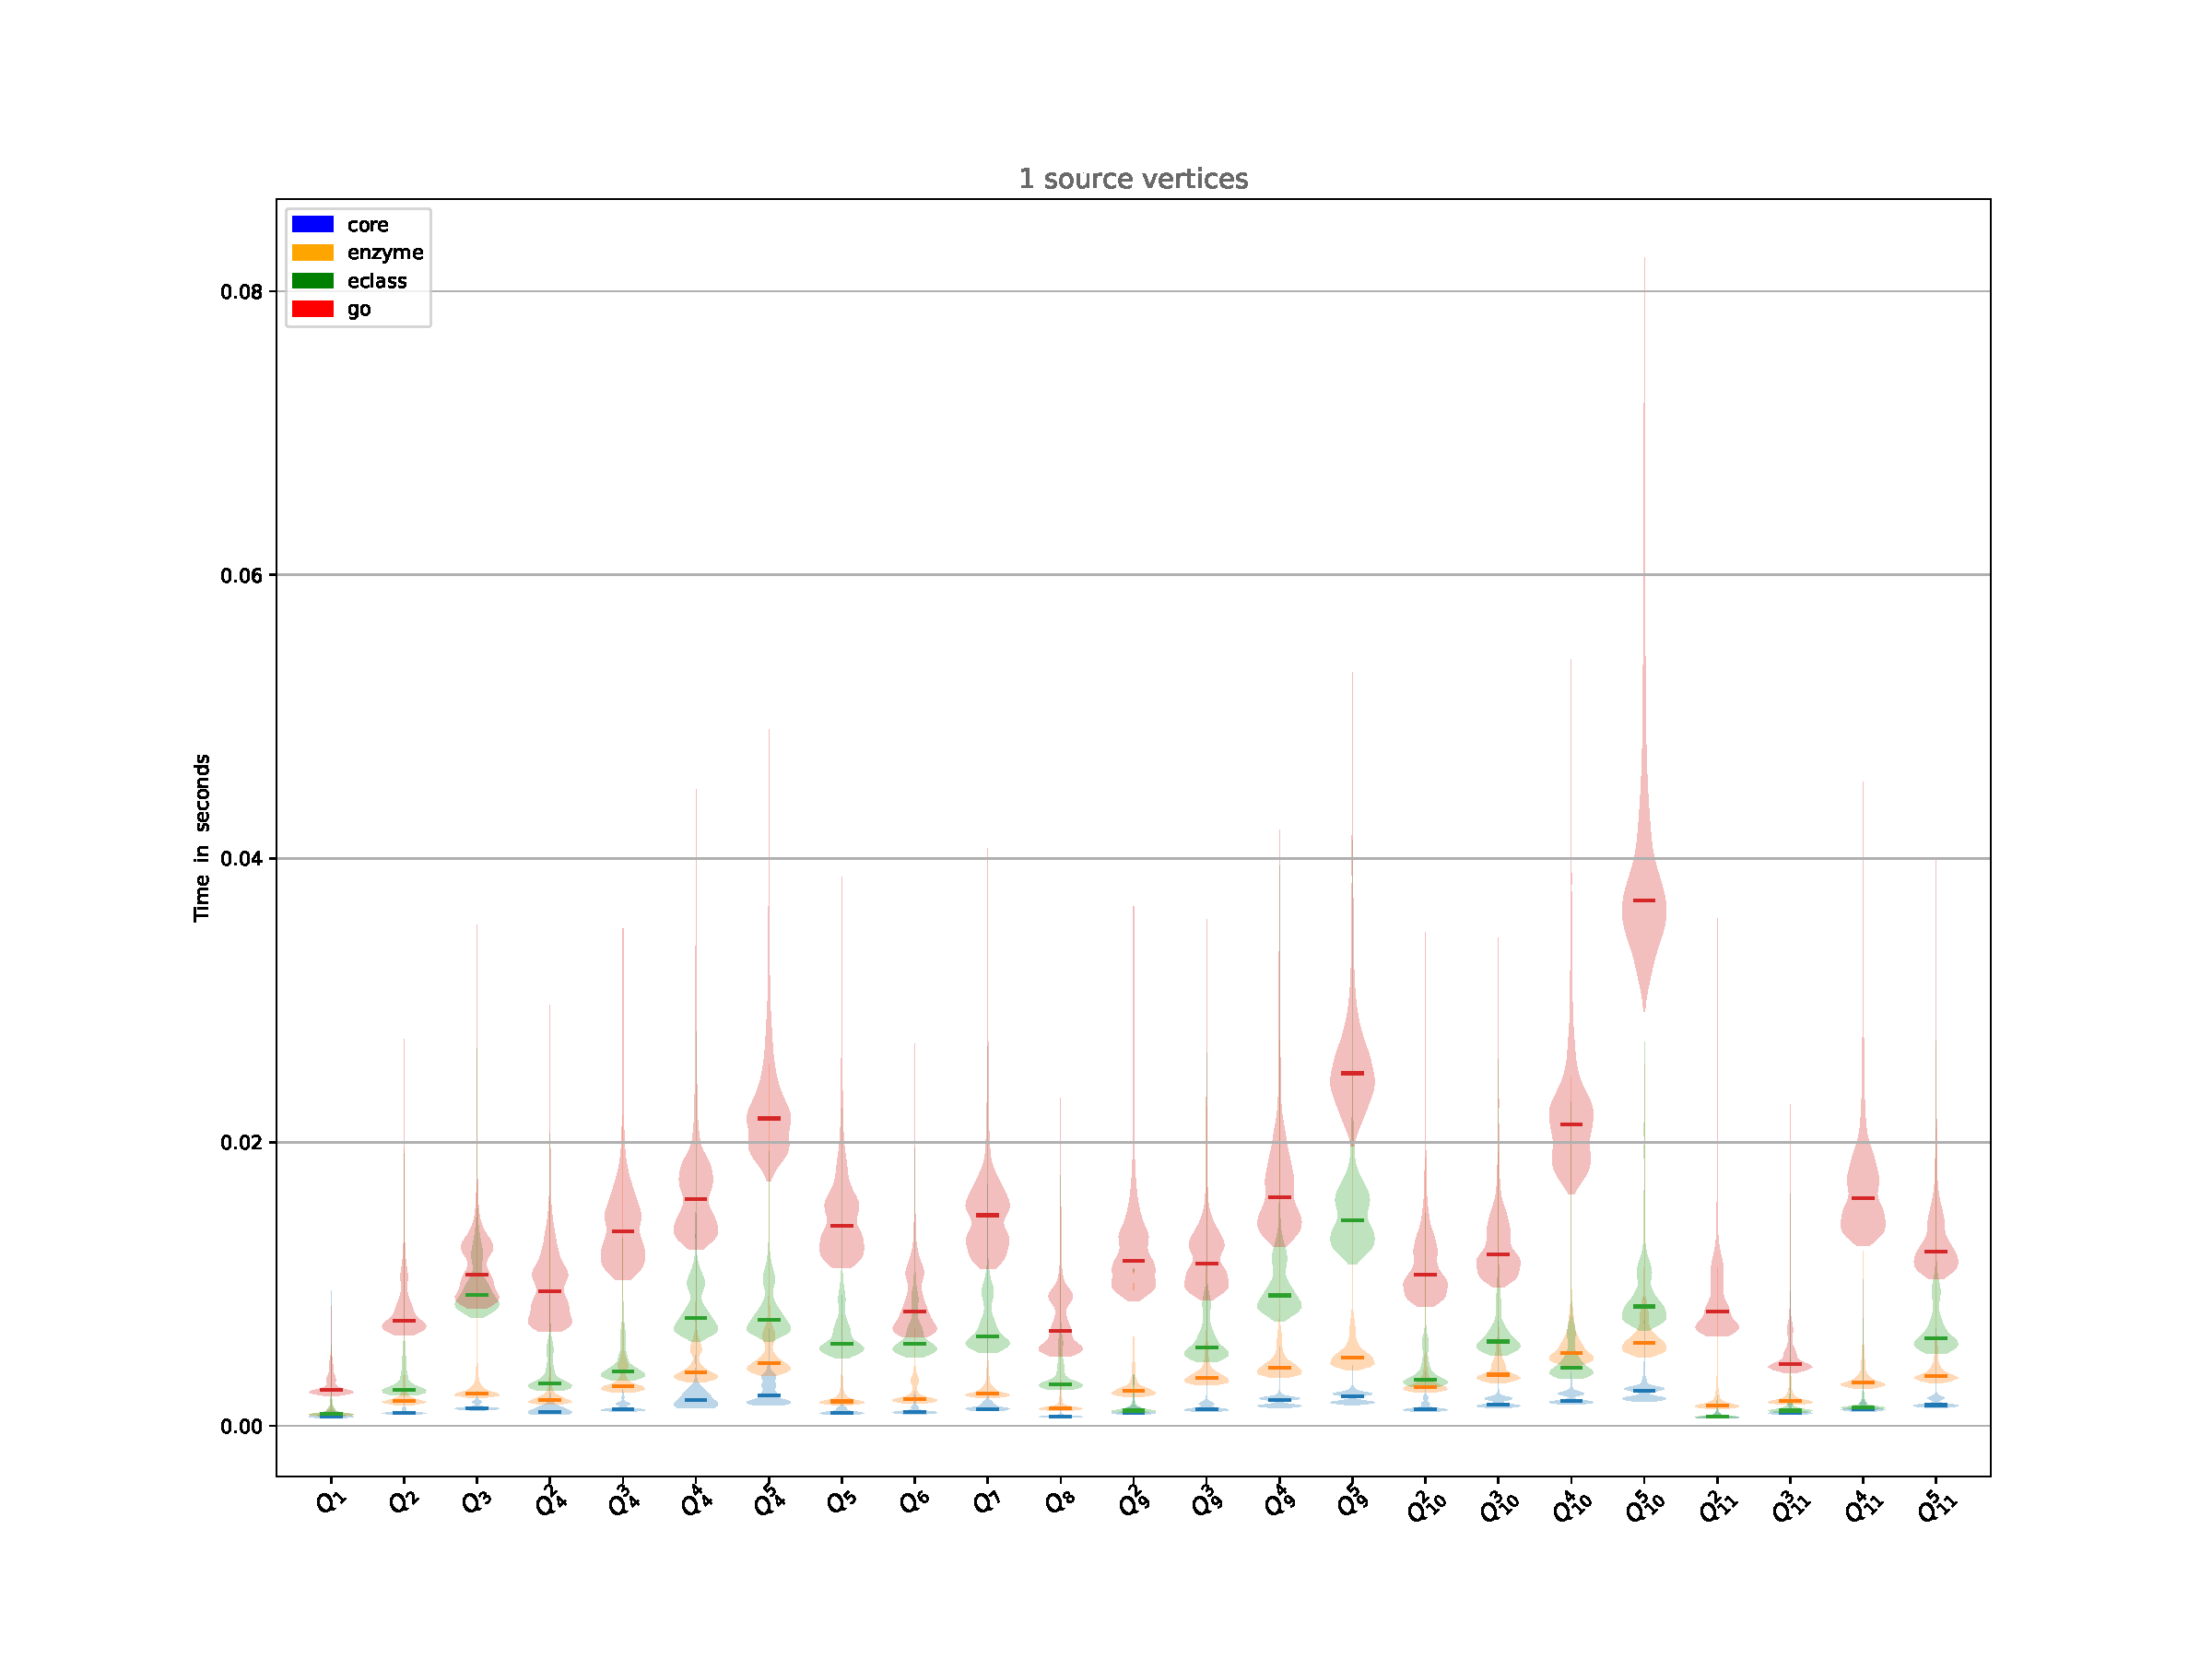
\includegraphics[width=1\linewidth]{pictures/ss1.pdf}
  \end{figure}
\end{minipage}
\end{frame}

\begin{frame}[fragile]
  \frametitle{Экспериментальное исследование (MS 1000)}
  \noindent\begin{minipage}{0.95\textwidth}
  \begin{figure}[h!]
      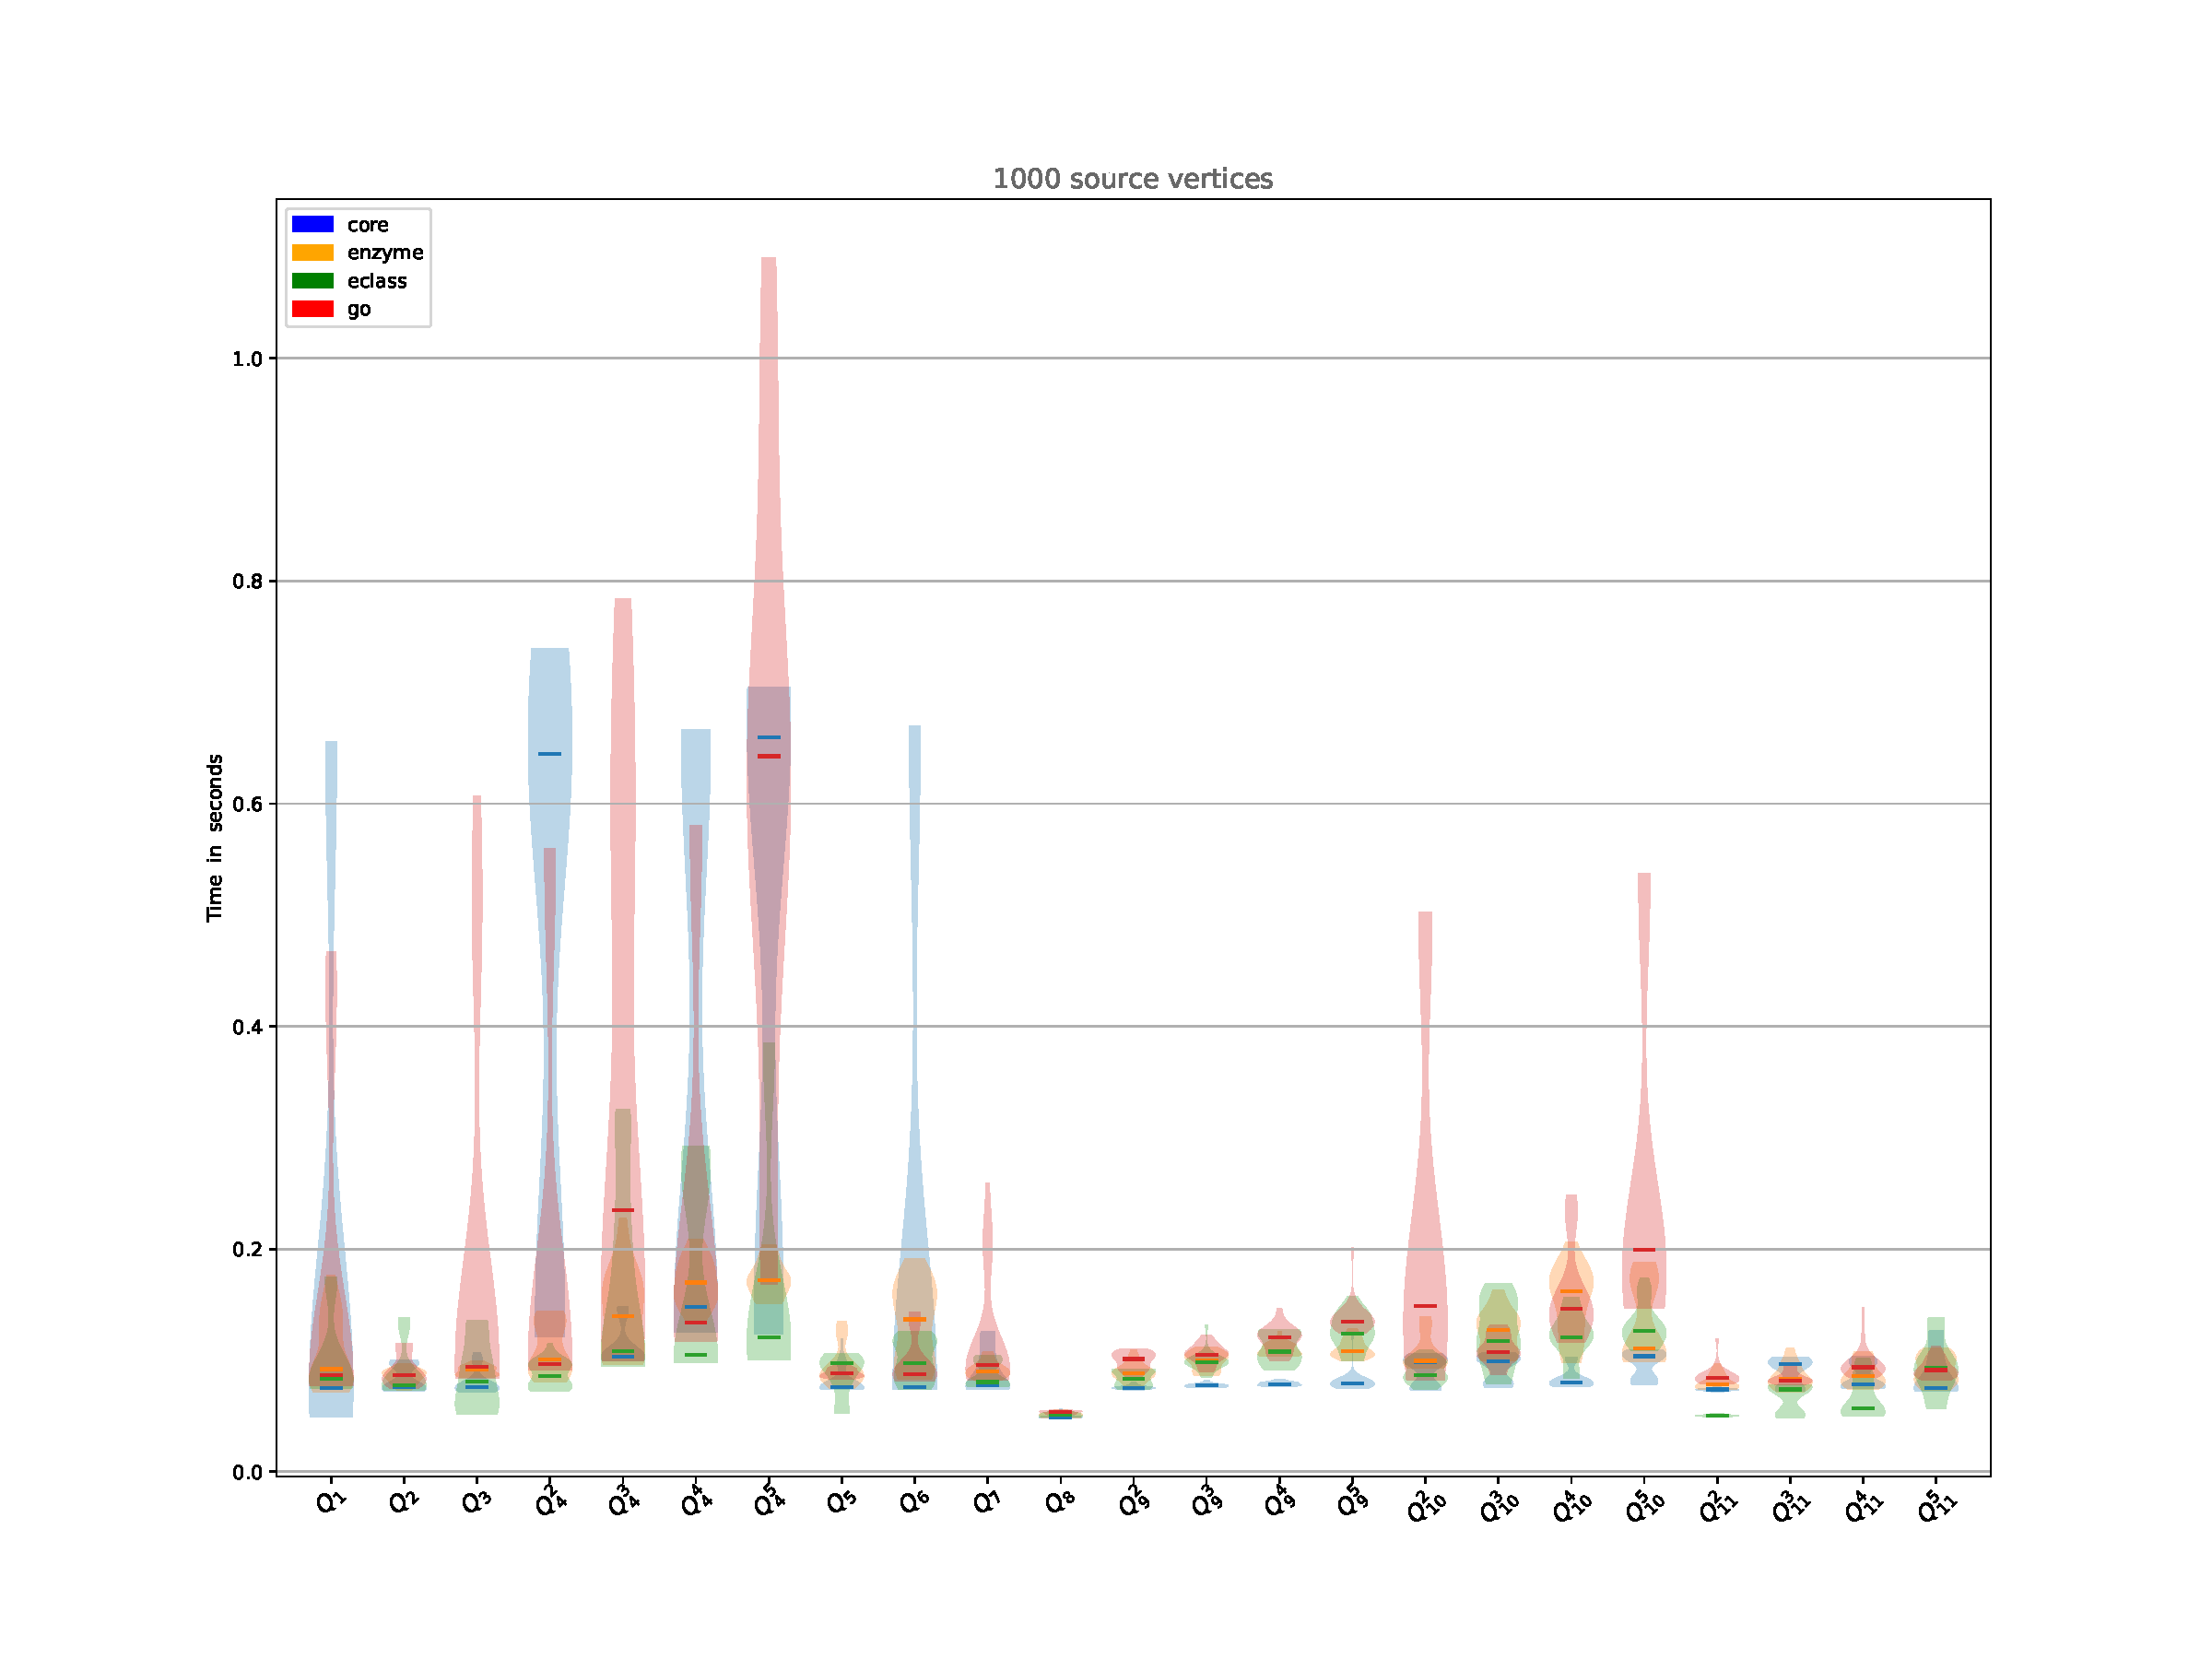
\includegraphics[width=1\linewidth]{pictures/ms1000.pdf}
  \end{figure}
\end{minipage}
\end{frame}

\begin{frame}
  \frametitle{Результаты}
  \begin{itemize}
    \item Проведен обзор основных методов и алгоритмов решения задачи регулярной достижимости 
    \item Разработан алгоритм, решающий задачу достижимости с регулярными ограничениями, в терминах линейной алгебры
    \item Реализован\footnote{\href{https://github.com/JetBrains-Research/CFPQ_PyAlgo/pull/34}{https://github.com/JetBrains-Research/CFPQ\_PyAlgo/pull/34}} разработанный алгоритм
    \item Проведено экспериментальное исследование алгоритма
  \end{itemize}
\end{frame}

\appendix

\begin{frame}[fragile]
  \frametitle{Алгоритм в псевдокоде}
  \begin{figure}[h!]
      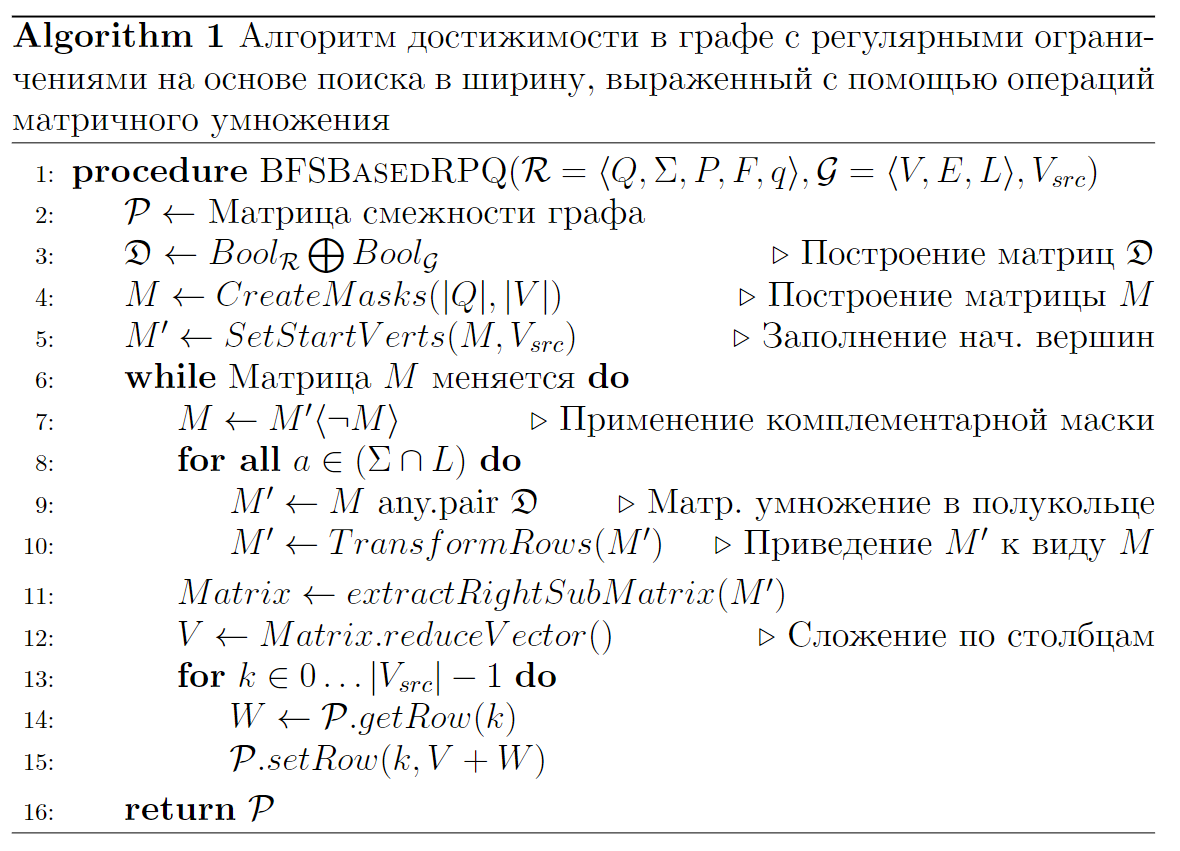
\includegraphics[width=0.9\linewidth]{pictures/pseudocode.PNG}
  \end{figure}
\end{frame}

\begin{frame}[fragile]
  \frametitle{Экспериментальное исследование (MS 10)}
  \noindent\begin{minipage}{0.95\textwidth}
  \begin{figure}[h!]
      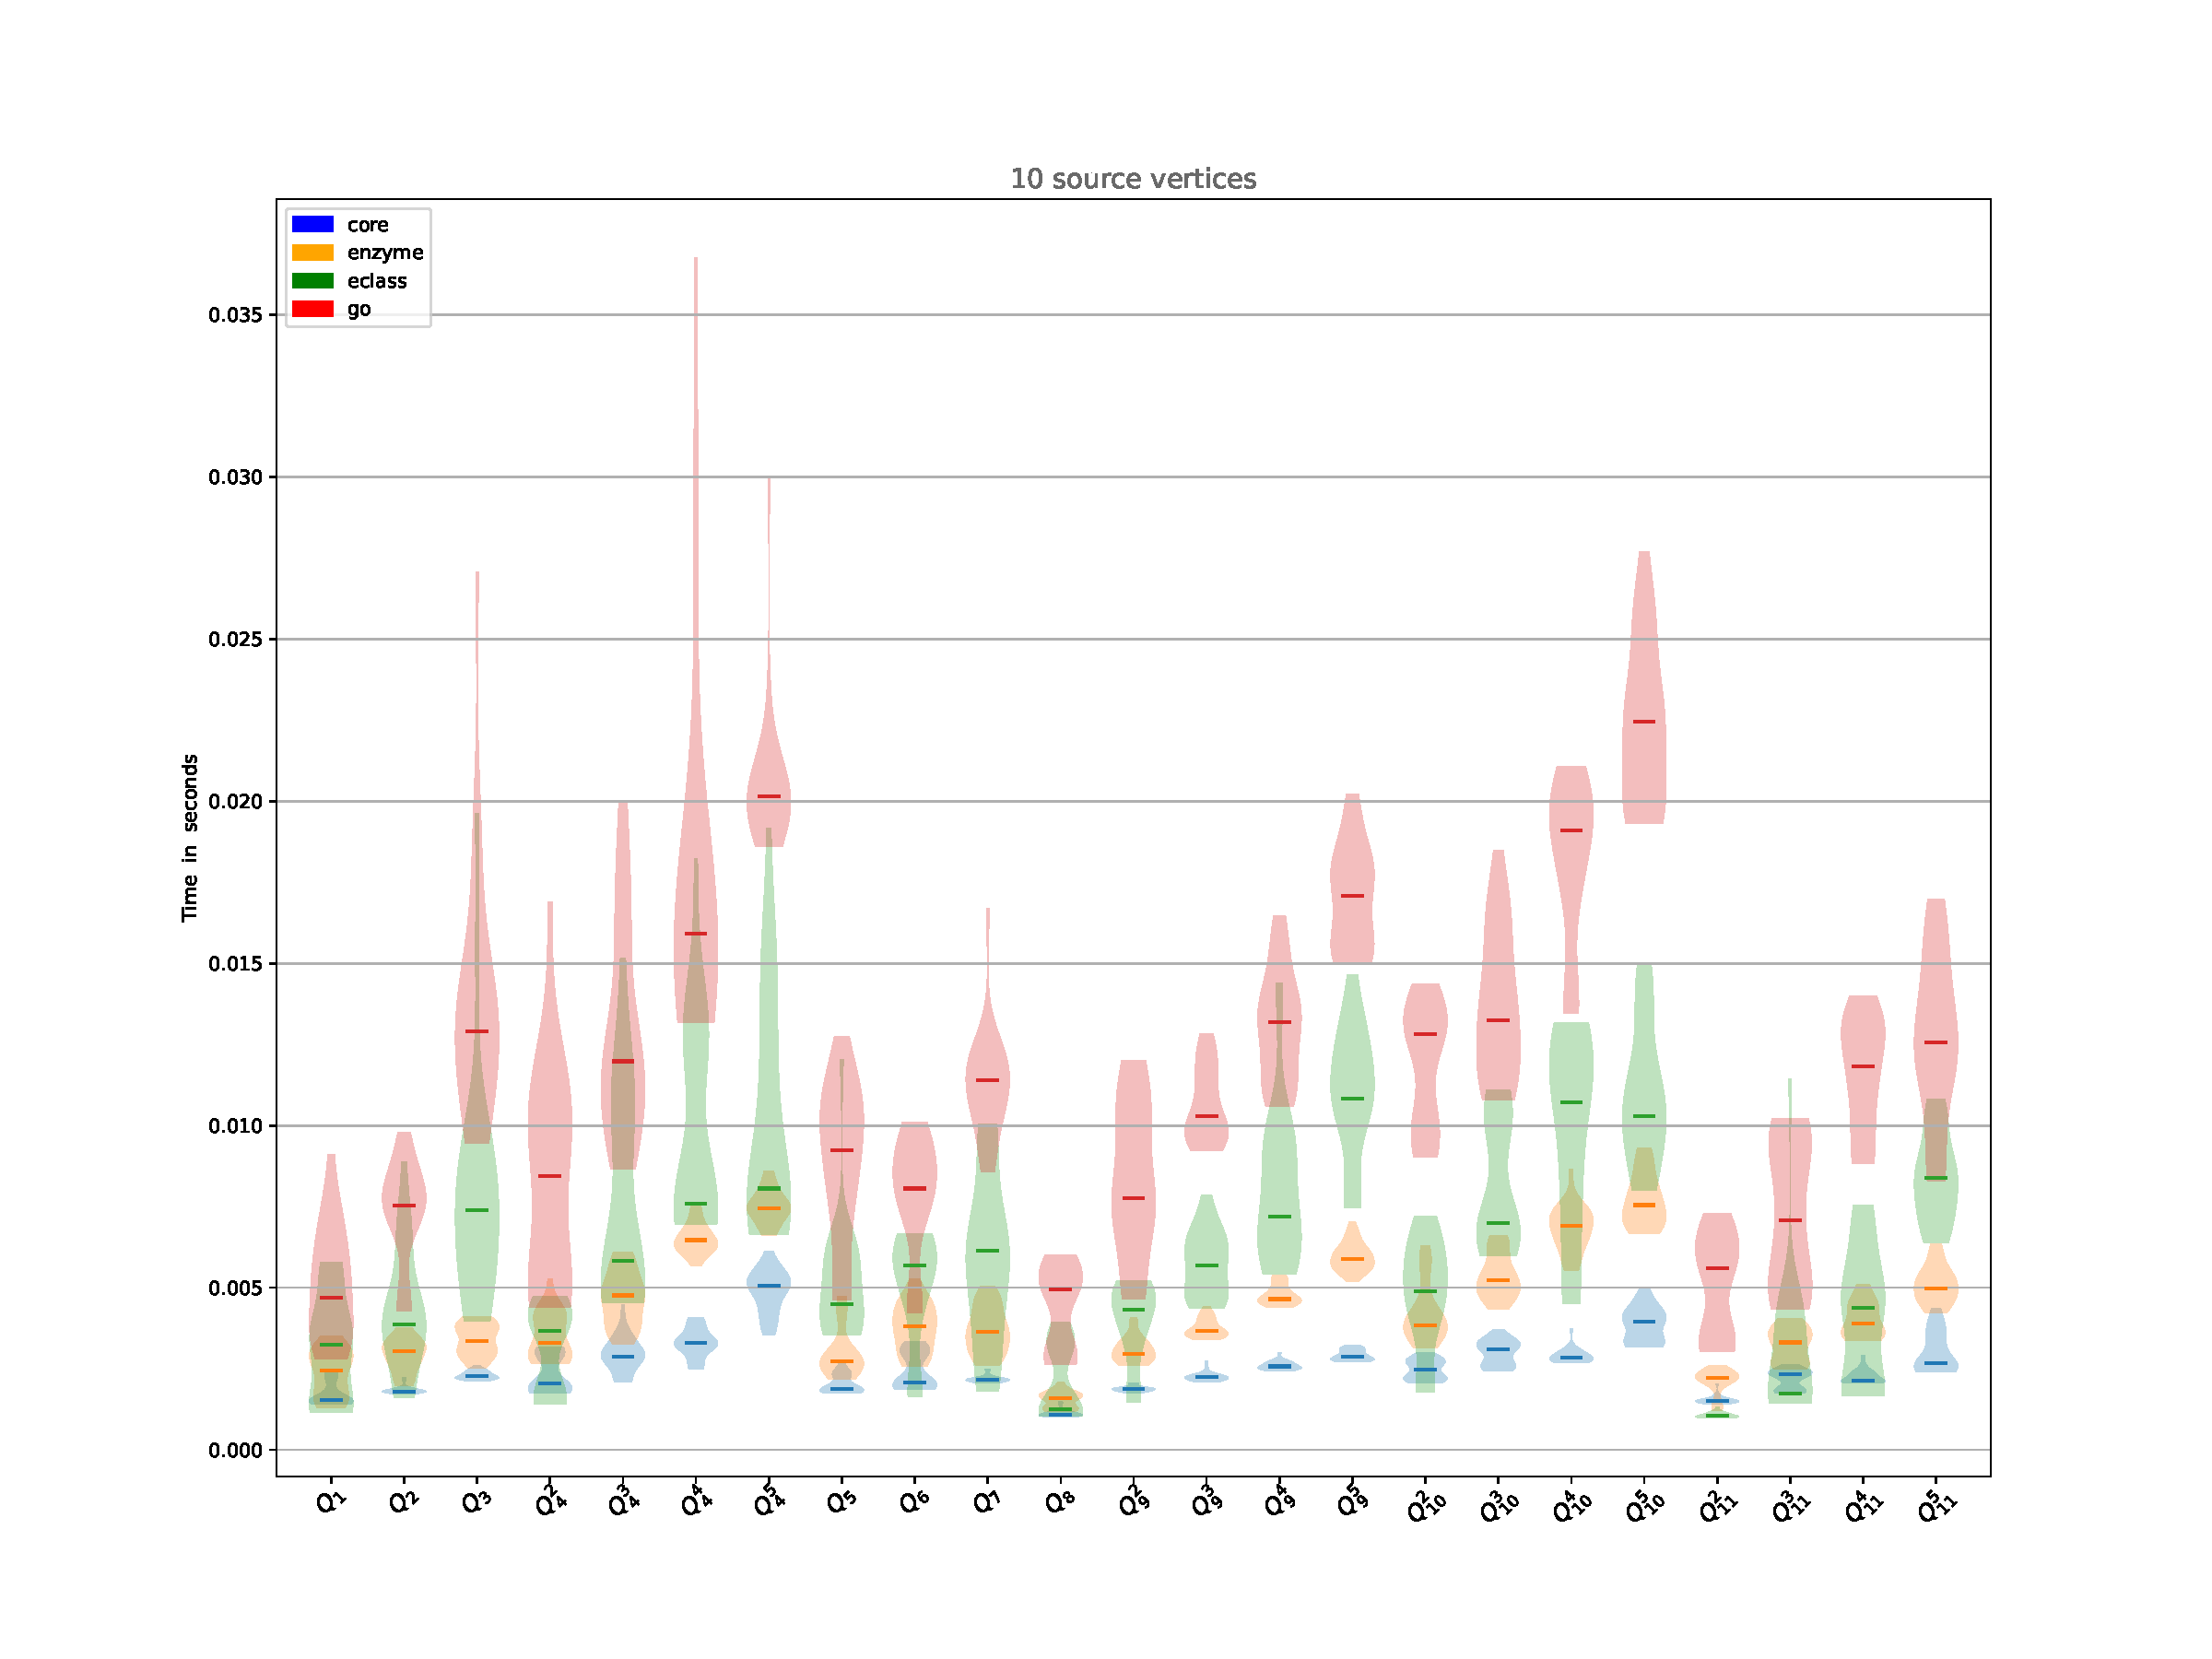
\includegraphics[width=1\linewidth]{pictures/ms10.pdf}
  \end{figure}
\end{minipage}
\end{frame}

\begin{frame}[fragile]
  \frametitle{Экспериментальное исследование (MS 100)}
  \noindent\begin{minipage}{0.95\textwidth}
  \begin{figure}[h!]
      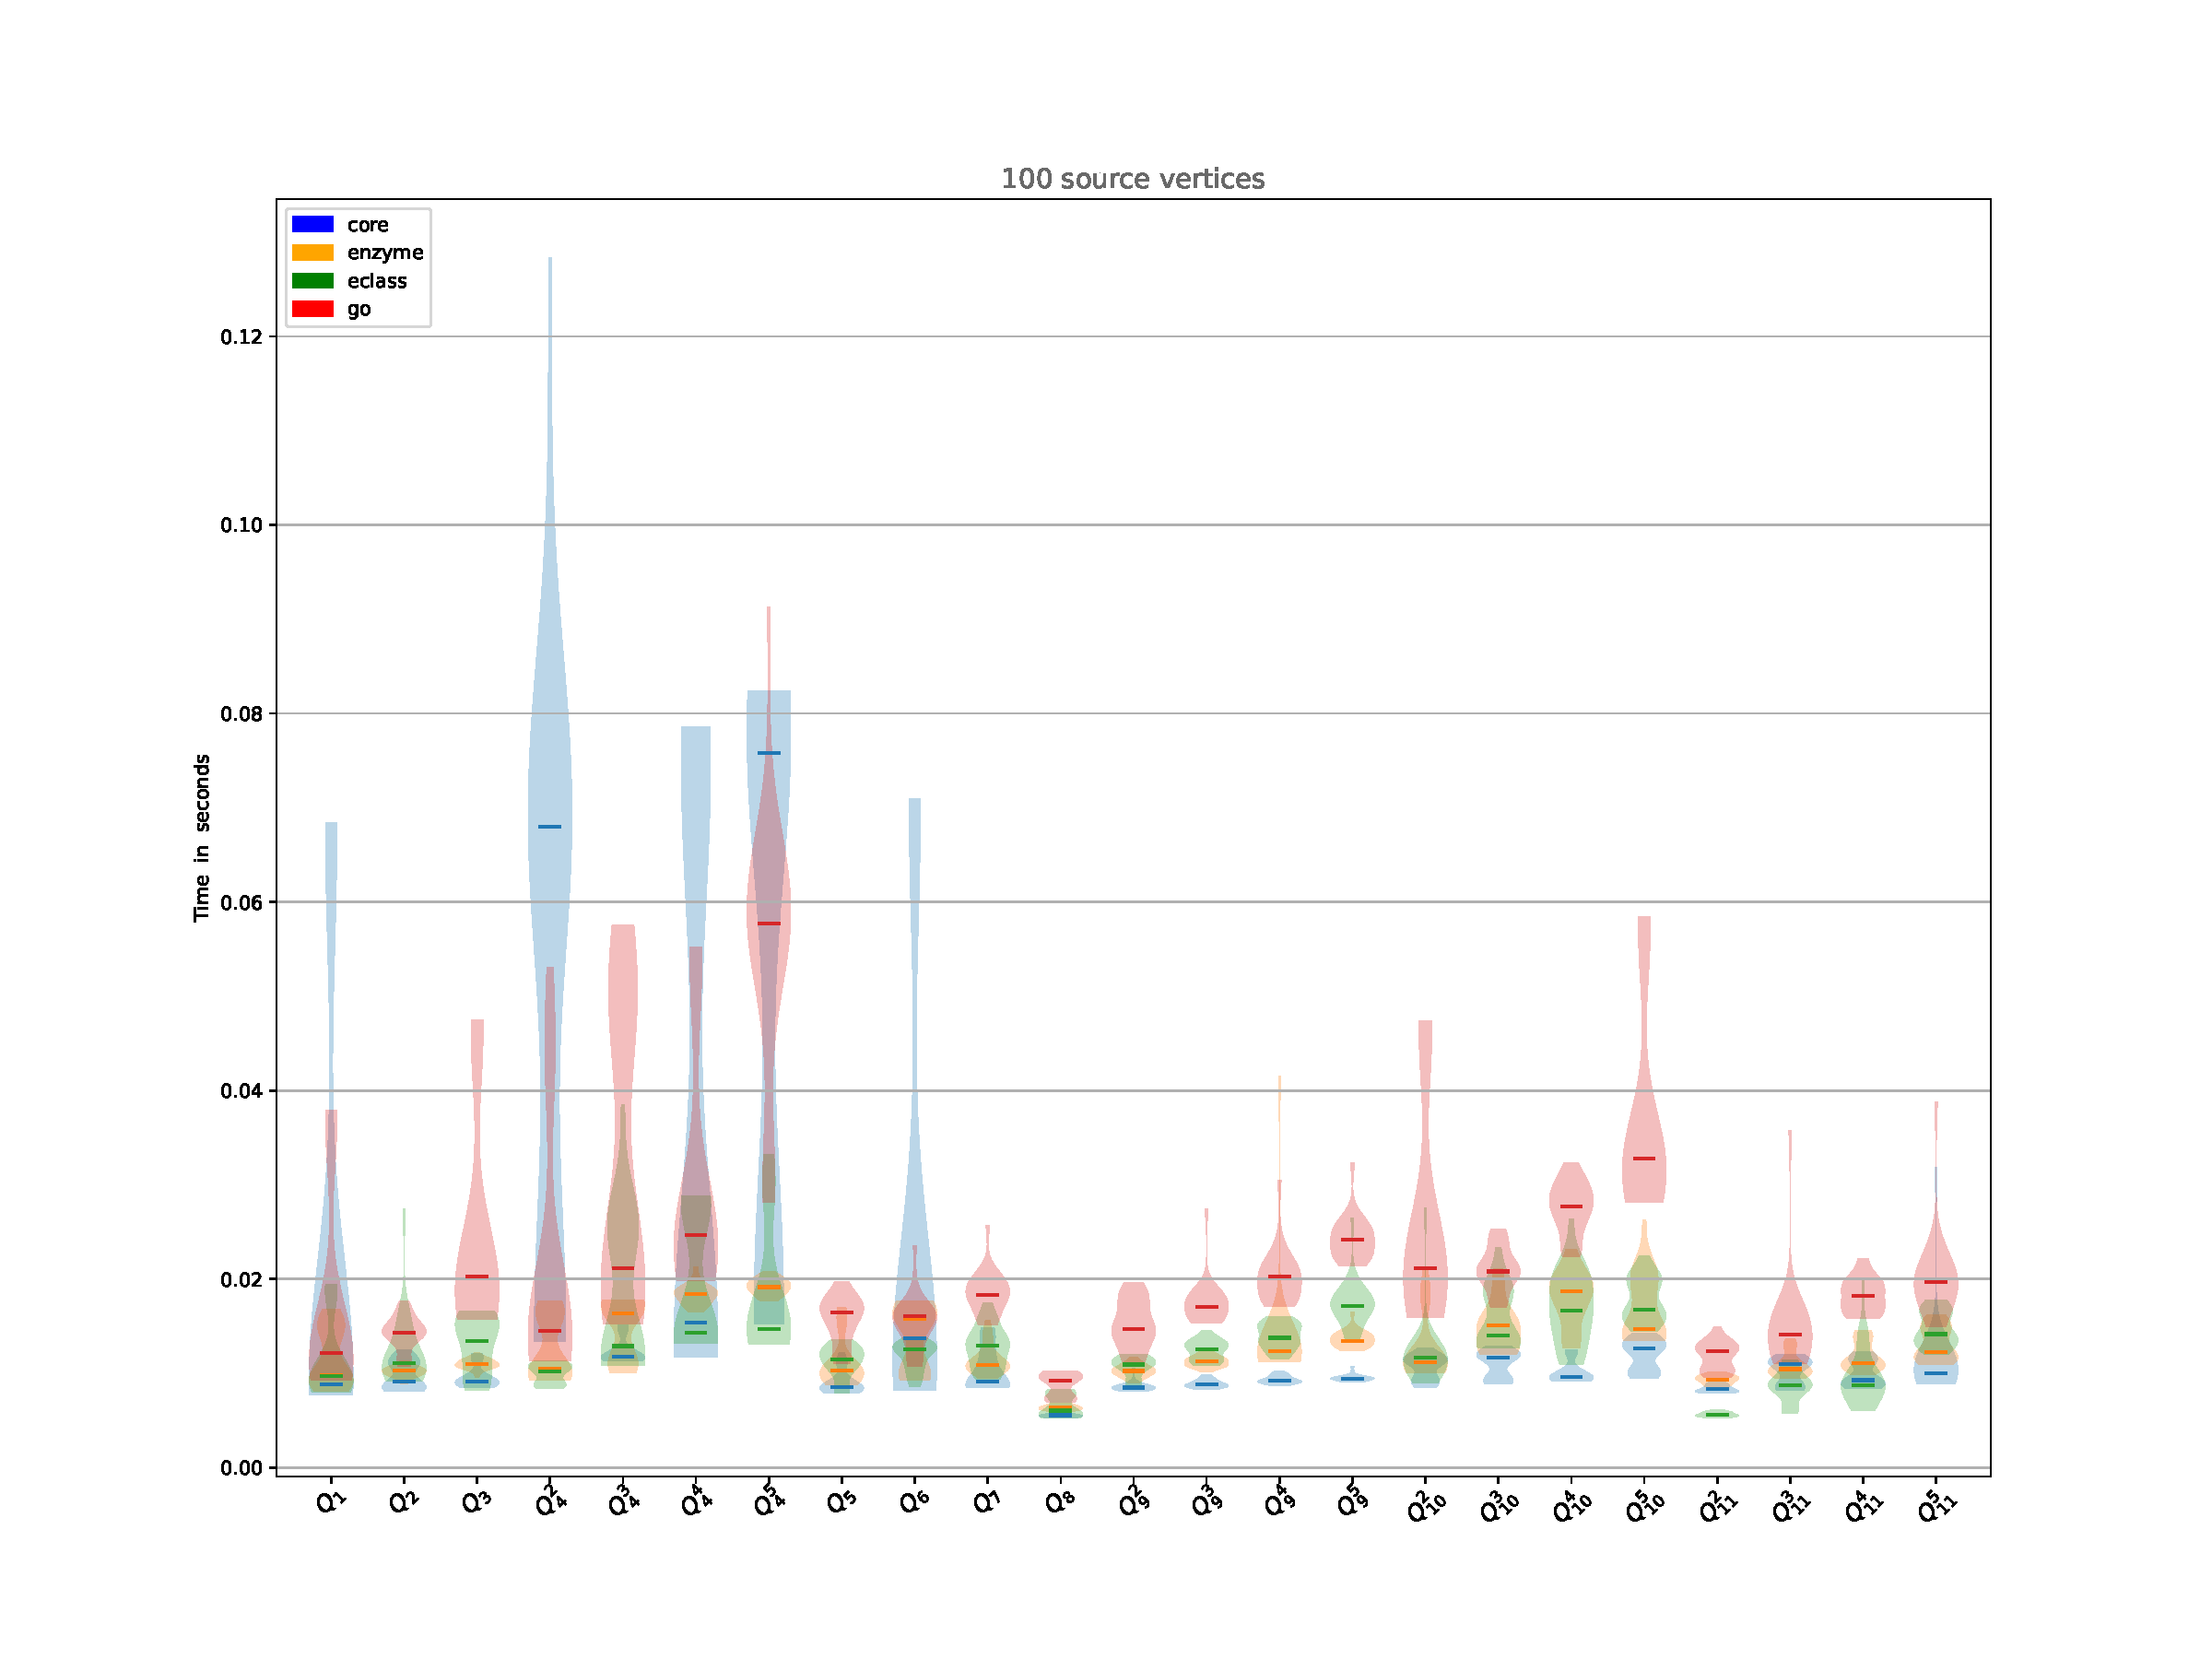
\includegraphics[width=1\linewidth]{pictures/ms100.pdf}
  \end{figure}
\end{minipage}
\end{frame}

\end{document}
